\newpage
\section{Models with default settings}

\subsection{Decision Tree}
Library function used: \texttt{\href{https://scikit-learn.org/stable/modules/generated/sklearn.tree.DecisionTreeClassifier.html}{DecisionTreeClassifier}} from \texttt{sklearn.tree}
\begin{table}[h!]
  \begin{minipage}{.5\linewidth}
    \centering
    \begin{tabular}{|l|c|}
      \hline
      \textbf{Parameter} & \textbf{Default Value} \\
      \hline
      \texttt{max\_depth} & None \\
      \texttt{min\_samples\_leaf} & 1 \\
      \texttt{min\_samples\_split} & 2 \\
      \hline
    \end{tabular}
    \caption{Default parameters}
  \end{minipage}%
  \begin{minipage}{.5\linewidth}
    \centering
    \begin{tabular}{|l|c|c|}
      \hline
      \textbf{Metric} & \textbf{Train} & \textbf{Test} \\
      \hline
      Accuracy & 100.0\% & 87.63\% \\
      Precision (macro) & 100.0\% & 87.5\% \\
      Recall (macro) & 100.0\% & 87.47\% \\
      F1-Score (macro) & 100.0\% & 87.48\% \\
      \hline
    \end{tabular}
    \caption{Performance Metrics}
  \end{minipage}
\end{table}


It is clear that Decision Trees cause overfitting, here especially because we didn't limit the depth of the tree.
\subsection{Random Forest}
Library function used: \texttt{\href{https://scikit-learn.org/stable/modules/generated/sklearn.ensemble.RandomForestClassifier.html}{RandomForestClassifier}} from \texttt{sklearn.ensemble}

\begin{table}[h!]
  \begin{minipage}{.5\linewidth}
    \centering
    \begin{tabular}{|l|c|}
      \hline
      \textbf{Parameter} & \textbf{Default Value} \\
      \hline
      \texttt{max\_depth} & None \\
      \texttt{min\_samples\_leaf} & 1 \\
      \texttt{min\_samples\_split} & 2 \\
      \texttt{n\_estimators} & 100 \\
      \hline
    \end{tabular}
    \caption{Default parameters}
  \end{minipage}%
  \begin{minipage}{.5\linewidth}
    \centering
    \begin{tabular}{|l|c|c|}
      \hline
      \textbf{Metric} & \textbf{Train} & \textbf{Test} \\
      \hline
      Accuracy & 100.0\% & 96.9\% \\
      Precision (macro) & 100.0\% & 96.88\% \\
      Recall (macro) & 100.0\% & 96.87\% \\
      F1-Score (macro) & 100.0\% & 96.87\% \\
      \hline
    \end{tabular}
    \caption{Performance Metrics}
  \end{minipage}
\end{table}


Random Forests give better test metrics than Decision Trees. Its important to note that they take longer to train.

\subsection{Na\"{i}ve Bayes Classifier}
Library function used: \texttt{\href{https://scikit-learn.org/stable/modules/generated/sklearn.naive_bayes.MultinomialNB.html}{MultinomialNB}} from \texttt{sklearn.naive\_bayes}
\begin{table}[h!]
  \begin{minipage}{.5\linewidth}
    \centering
    \begin{tabular}{|l|c|}
      \hline
      \textbf{Parameter} & \textbf{Default Value} \\
      \hline
      \texttt{No parameters to tune} & N/A \\
      \hline
    \end{tabular}
    \caption{Default parameters}
  \end{minipage}%
  \begin{minipage}{.5\linewidth}
    \centering
    \begin{tabular}{|l|c|c|}
      \hline
      \textbf{Metric} & \textbf{Train} & \textbf{Test} \\
      \hline
      Accuracy & 82.46\% & 83.57\% \\
      Precision (macro) & 83.15\% & 84.29\% \\
      Recall (macro) & 82.16\% & 83.26\% \\
      F1-Score (macro) & 82.32\% & 83.42\% \\
      \hline
    \end{tabular}
    \caption{Performance Metrics}
  \end{minipage}
\end{table}

Na\"{i}ve Bayes performs poorest. This is likely under-fitting. For image data, the \textbf{naive} assumption fails miserably as pixel values are highly correlated when near. 

\subsection{KNN Classifier}
Library function used: \texttt{\href{https://scikit-learn.org/stable/modules/generated/sklearn.neighbors.KNeighborsClassifier.html}{KNeighborsClassifier}} from \texttt{sklearn.neighbors}

\begin{table}[h!]
  \begin{minipage}{.5\linewidth}
    \centering
    \begin{tabular}{|l|c|}
      \hline
      \textbf{Parameter} & \textbf{Default Value} \\
      \hline
      \texttt{n\_neighbors} & 5 \\
      \texttt{weights} & uniform \\
      \hline
    \end{tabular}
    \caption{Default parameters}
  \end{minipage}%
  \begin{minipage}{.5\linewidth}
    \centering
    \begin{tabular}{|l|c|c|}
      \hline
      \textbf{Metric} & \textbf{Train} & \textbf{Test} \\
      \hline
      Accuracy & 98.19\% & 96.88\% \\
      Precision (macro) & 98.22\% & 96.93\% \\
      Recall (macro) & 98.16\% & 96.85\% \\
      F1-Score (macro) & 98.19\% & 96.87\% \\
      \hline
    \end{tabular}
    \caption{Performance Metrics}
  \end{minipage}
\end{table}

\newpage
\subsection{Neural Network Classifier}
Library function used: \texttt{\href{https://www.tensorflow.org/api_docs/python/tf/keras/Layer}{Layer}, \href{https://www.tensorflow.org/api_docs/python/tf/keras/Model}{Model}} from \texttt{tensorflow.keras}

\begin{table}[h!]
  \begin{minipage}{.5\linewidth}
    \centering
    \begin{tabular}{|l|c|}
      \hline
      \textbf{Parameter} & \textbf{Default Value} \\
      \hline
      \texttt{activation} & relu \\
      \texttt{alpha} & 0.0001 \\
      \texttt{hidden\_layer\_sizes} & 100 \\
      \texttt{epochs} & 5 \\
      \hline
    \end{tabular}
    \caption{Default parameters}
  \end{minipage}%
  \begin{minipage}{.5\linewidth}
    \centering
    \begin{tabular}{|l|c|c|}
      \hline
      \textbf{Metric} & \textbf{Train} & \textbf{Test} \\
      \hline
      Accuracy & 99.12\% & 97.62\% \\
      Precision (macro) & 99.13\% & 97.63\% \\
      Recall (macro) & 99.12\% & 97.60\% \\
      F1-Score (macro) & 99.12\% & 97.60\% \\
      \hline
    \end{tabular}
    \caption{Performance Metrics}
  \end{minipage}
\end{table}


One \verb|epoch| is one single run over the entire training data. Neural Network, with these settings give the best \verb|test| accuracy in models shown above.

\begin{figure}[h!]
    \centering
    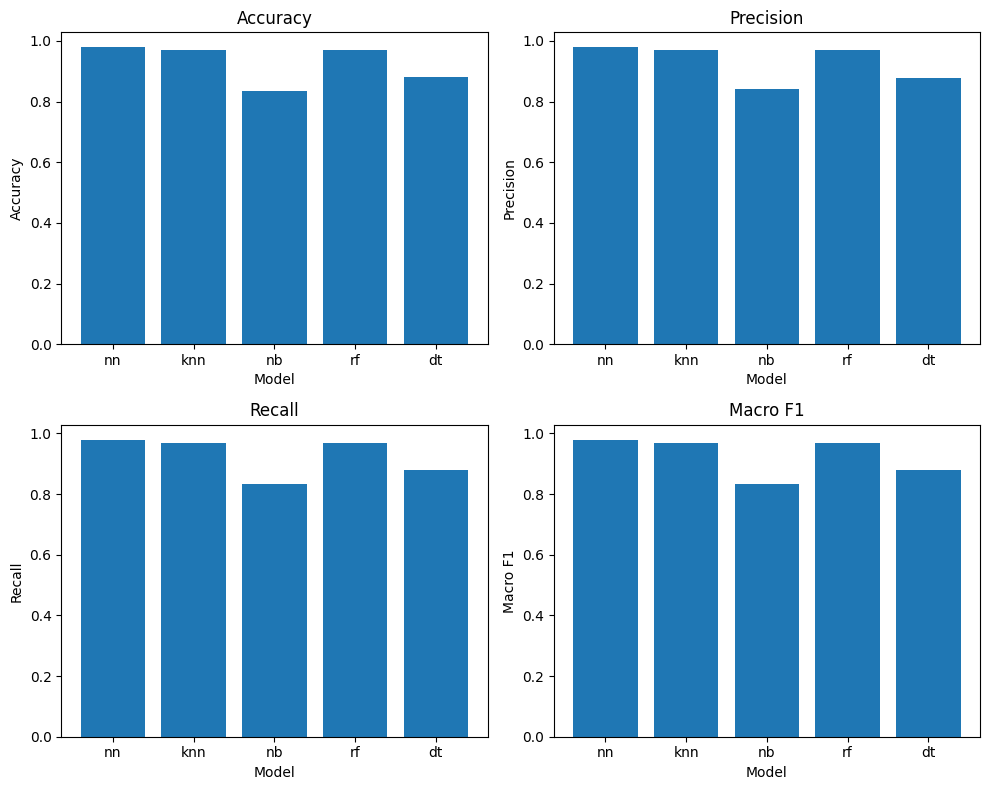
\includegraphics[width=0.8\linewidth]{images/acc_models.png}
    \caption{Metrics on test set for various models}
\end{figure}